
工程师不喜欢体力劳动,某件事可以自动化,就可能会自动化。通过所有这些努力来创建足够好的文档,要是能实现部分工作的自动化实际上也是一种福报。

\subsubsubsection{3.8.1\hspace{0.2cm}生成需求文档}

如果从零开始创建一个项目,可能很难凭空生成文档。若相应的工具中有需求,那么还可以生成文档。例如,正在使用JIRA,起点应该是从问题导航器视图中导出所有项。可以使用过滤器,并只获相应项目的打印输出。如果不喜欢默认的字段集,或者觉得不是想要的,可以尝试JIRA的需求管理插件,可以导出需求,例如:\textbf{R4J(Requirements for Jira)}允许创建需求的整个层次结构,并进行跟踪,管理更改,并在整个项目中进行传播,执行需求更改的影响分析。当然,可以使用用户定义的模板导出。许多这样的工具也可以为需求创建测试套件,但目前没有免费的版本。

\subsubsubsection{3.8.2\hspace{0.2cm}用代码中生成图表}

如果想在不深入源代码的情况下了解代码结构,可能会对代码生成图表的工具感兴趣。

CppDepend就是这样一个工具,能够在不同的源码间创建各种依赖关系图。更重要的是,允许通过各种参数查询和过滤代码。无论只是想了解代码的结构、发现不同软件组件之间的依赖关系,以及它们耦合的紧密程度,还是想快速定位技术负担最重的部分,这个工具都能有所帮助。这个软件需要花钱,但提供试用版本。

有些绘图工具可以从类图创建代码,从代码创建类图。企业版能够获得类图和接口图,并以多种语言生成代码。C++就是其中之一,可以直接从源代码生成UML类图。另一个可以完成这项任务的工具是Visual Paradigm。

\subsubsubsection{3.8.3\hspace{0.2cm}用代码生成(API)文档}

为了帮助其他人浏览现有代码,并使用提供的API,好的方法是提供从代码中的注释生成的文档。这类文档最好就放在所描述的函数和数据类型旁边,这有助于保持同步。

编写此类文档的标准工具是Doxygen,优点是速度快(特别是对于大型项目和HTML文档生成),生成器有一些内置的正确性检查(例如,对于函数中部分记录的参数—检查文档是否是最新版本,可以有一个很好的标记),并且它允许对类和文件层次结构进行导航。缺点包括不能进行全文搜索,生成的PDF不够理想,界面操作可能有点麻烦。

幸运的是,可用性缺陷可以通过使用另一个文档工具来弥补。如果曾经阅读过Python文档,那么可能遇到过Sphinx。它的外观新颖、可用比较好的界面,并使用reStructuredText作为标记语言。好消息是,在这两者之间有一个桥梁,因此可以使用Doxygen生成的XML并在Sphinx中使用它。这个桥接软件叫做Breathe。

现在看看如何在项目中进行设置。假设将源代码保存在\textit{src}中,公共头文件保存在\textit{include}中,文档保存在\textit{doc}中。首先,创建一个\textit{CMakeLists.txt}文件:

\begin{lstlisting}[style=styleCMake]
cmake_minimum_required(VERSION 3.10)

project("Breathe Demo" VERSION 0.0.1 LANGUAGES CXX)

list(APPEND CMAKE_MODULE_PATH "${CMAKE_CURRENT_LIST_DIR}/cmake")
add_subdirectory(src)
add_subdirectory(doc)
\end{lstlisting}

对项目支持的CMake版本设置了要求,指定了名称、版本和使用的语言(在例子中,只有C++),并将\textit{CMake}目录添加到CMake查找包含文件的路径中。

\textit{cmake}子目录中,创建一个文件\textit{FindSphin.cmake},这里直接使用它的名字,因为Sphinx还没有提供相应的cmake文件:

\begin{lstlisting}[style=styleCMake]
find_program(
	SPHINX_EXECUTABLE
	NAMES sphinx-build
	DOC "Path to sphinx-build executable")

# handle REQUIRED and QUIET arguments, set SPHINX_FOUND variable
include(FindPackageHandleStandardArgs)
find_package_handle_standard_args(
  Sphinx "Unable to locate sphinx-build executable" SPHINX_EXECUTABLE)
\end{lstlisting}

现在,CMake将查找Sphinx构建工具。如果找到,将设置适当的CMake变量,将Sphinx包标记为已找到。接下来,创建源文件来生成文档。创建一个\textit{include/breathe\_demo/demo.h}文件:

\begin{lstlisting}[style=styleCXX]
#pragma once

// the @file annotation is needed for Doxygen to document the free
// functions in this file
/**
* @file
* @brief The main entry points of our demo
*/

/**
* A unit of performable work
*/
struct Payload {
	/**
	* The actual amount of work to perform
	*/
	int amount;
};

/**
	@brief Performs really important work
	@param payload the descriptor of work to be performed
*/
void perform_work(struct Payload payload);
\end{lstlisting}

注意注释语法。Doxygen在解析头文件时识别它,以便知道在生成的文档中放入什么。

现在,为头文件添加一个相应的\textit{src/demo.cpp}实现:

\begin{lstlisting}[style=styleCXX]
#include "breathe_demo/demo.h"

#include <chrono>
#include <thread>

void perform_work(Payload payload) {
	std::this_thread::sleep_for(std::chrono::seconds(payload.amount));
}	
\end{lstlisting}

这里没有Doxygen的注释。更倾向于在头文件中记录类型和函数,因为它们是库接口。源文件只是实现,它们没有向接口添加新内容。

除了前面的文件,还需要在\textit{src}中放一个简单的\textit{CMakeLists.txt}:

\begin{lstlisting}[style=styleCMake]
add_library(BreatheDemo demo.cpp)
target_include_directories(BreatheDemo PUBLIC
	${PROJECT_SOURCE_DIR}/include)
target_compile_features(BreatheDemo PUBLIC cxx_std_11)
\end{lstlisting}

这里,指定目标的源文件、包含目标头文件的目录,以及编译所需的C++标准。

现在,移动到\textit{doc}文件夹。\textit{CMakeLists.txt}文件首先检查Doxygen是否可用,如果可用则省略生成:

\begin{lstlisting}[style=styleCMake]
find_package(Doxygen)
if (NOT DOXYGEN_FOUND)
	return()
endif()
\end{lstlisting}

如果没有安装Doxygen,将跳过文档生成。还要注意\textit{return()}会退出当前的CMake文件,这是一个并不广为人知,但有用的技巧。

接下来,假设发现了Doxygen,需要设置一些变量来控制生成。这里只想要Breathe的XML输出,所以需要设置以下变量:

\begin{lstlisting}[style=styleCMake]
set(DOXYGEN_GENERATE_HTML NO)
set(DOXYGEN_GENERATE_XML YES)
\end{lstlisting}

要强制使用相对路径,可以使用\texttt{set(DOXYGEN\_STRIP\_FROM\_PATH \$\{PROJECT\_SOURCE\_DIR\}/include)}。如果实现细节需要隐藏,可以使用\texttt{set(DOXYGEN\_EXCLUDE\_PATTERNS "*/detail/*")}来实现。已经设置好了所有的变量,现在进行生成:

\begin{lstlisting}[style=styleCMake]
# Note: Use doxygen_add_docs(doxygen-doc ALL ...) if you want your
# documentation to be created by default each time you build. Without the 
# keyword you need to explicitly invoke building of the 'doc' target.
doxygen_add_docs(doxygen-doc ${PROJECT_SOURCE_DIR}/include COMMENT
	"Generating API documentation with Doxygen")
\end{lstlisting}

这里,调用专门为使用Doxygen编写的CMake函数。定义了一个目标,\textit{doxygen-doc},需要显式地调用它,按需生成文档,就像注释所述。

现在创建一个Breathe目标来使用Doxygen。可以使用\textit{FindSphinx}模块来完成这个任务:

\begin{lstlisting}[style=styleCMake]
find_package(Sphinx REQUIRED)
configure_file(${CMAKE_CURRENT_SOURCE_DIR}/conf.py.in
	${CMAKE_CURRENT_BINARY_DIR}/conf.py @ONLY)
add_custom_target(
	sphinx-doc ALL
	COMMAND ${SPHINX_EXECUTABLE} -b html -c ${CMAKE_CURRENT_BINARY_DIR}
	${CMAKE_CURRENT_SOURCE_DIR} ${CMAKE_CURRENT_BINARY_DIR}
	WORKING_DIRECTORY ${CMAKE_CURRENT_BINARY_DIR}
	COMMENT "Generating API documentation with Sphinx"
	VERBATIM)
\end{lstlisting}

首先,调用模块。然后,用项目中的变量填充一个Python配置文件,以便Sphinx使用。再创建了一个\textit{sphinx-doc}目标,它将生成HTML文件作为输出,并在这样做时在构建输出中打印一行。

最后,强制CMake在每次生成Sphinx文档时调用Doxygen:\texttt{add\_dependencies(sphinx-doc doxygen-doc)}.

如果希望为文档提供更多的目标,引入一些CMake函数可能会有用,这些函数将处理与文档相关的目标。

现在来看看\textit{conf.py.in}文件中,用来引导的工具。创建它,将其指向Sphinx:

\begin{lstlisting}[style=stylePython]
extensions = [ "breathe", "m2r2" ]
breathe_projects = { "BreatheDemo": "@CMAKE_CURRENT_BINARY_DIR@/xml" }
breathe_default_project = "BreatheDemo"

project = "Breathe Demo"
author = "Breathe Demo Authors"
copyright = "2021, Breathe Demo Authors"
version = "@PROJECT_VERSION@"
release = "@PROJECT_VERSION@"

html_theme = 'sphinx_rtd_theme'
\end{lstlisting}

从前面的清单中可以看到,设置了Sphinx要使用的扩展、文档记录项目的名称和其他一些相关变量。注意\texttt{@NOTATION@},由CMake使用适当的变量值填充输出文件。最后,告诉Sphinx使用ReadTheDocs主题(\texttt{Sphinx\_rtd\_theme})。

困难的最后一部分是reStructuredText文件,它定义了在文档的什么地方包含什么。首先,创建一个\textit{index.rst}文件,包含一个目录和一些链接:

\begin{tcblisting}{commandshell={}}
Breathe Demo
============

Welcome to the Breathe Demo documentation!
.. toctree::
    :maxdepth: 2
    :caption: Contents:
   
Introduction <self>
    readme
    api_reference
\end{tcblisting}

第一个链接指向这个页面,并且可以从其他页面返回到它。显示\textit{Introduction}作为标签,其他名称指向带有\textit{.rst}扩展。因为包含了M2R2 Sphinx扩展,所以可以在文档中包含\textit{README.md}文件,这样可以避免自述文件内容的重复,其实\textit{readme.rst}文件就是\textit{..mdinclude:: ../README.md}。现在进行最后一步:合并Doxygen的输出,使用下面的命令在\textit{api\_reference.rst}中完成:

\begin{tcblisting}{commandshell={}}
API Reference
=============

.. doxygenindex::

\end{tcblisting}

因此,目前只是按自己喜欢的方式命名了参考页面,并指定Doxygen生成的文档应该列在这里,就是这样!只要构建\textit{sphinx-doc}目标,会得到一个这样的页面:

\begin{center}
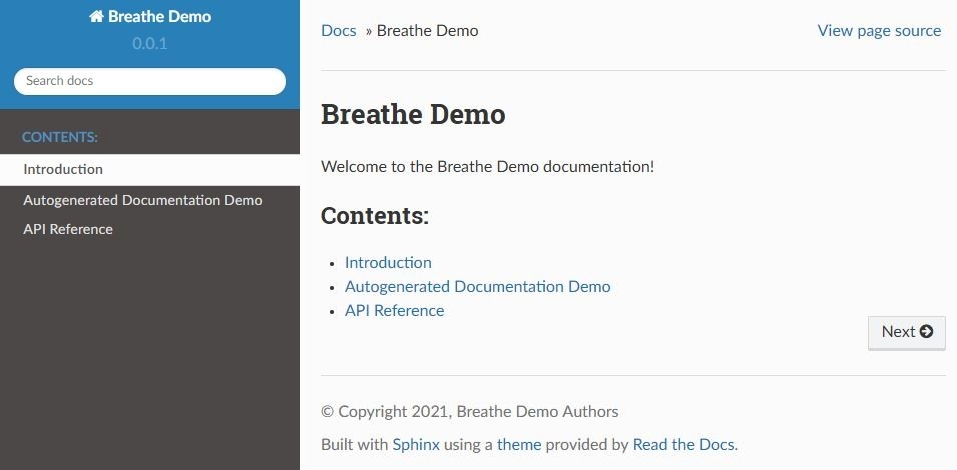
\includegraphics[width=0.9\textwidth]{content/1/chapter3/images/9.jpg}\\
图3.9 -文档的主页,合并了生成的和手工编写的部分
\end{center}

查看API文档页面时,应该是这样:

\begin{center}
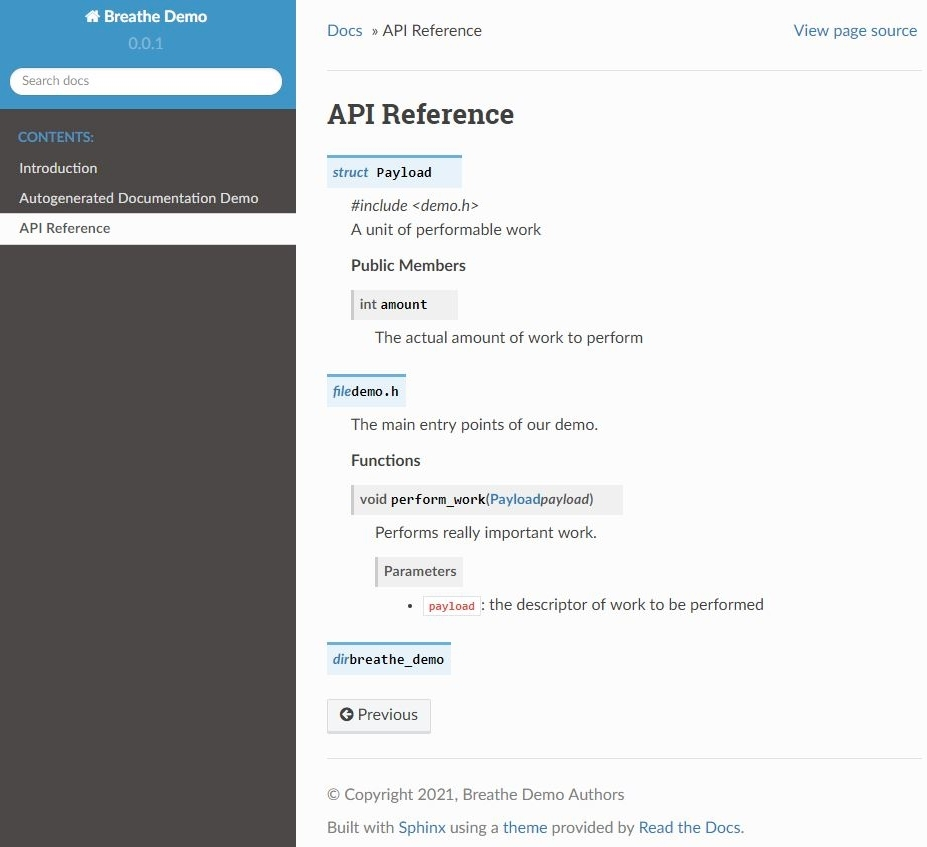
\includegraphics[width=0.9\textwidth]{content/1/chapter3/images/10.jpg}\\
图3.10 -自动生成的API文档
\end{center}

可以看到,文档是为我们的\textit{Payload}类型自动生成的,它的每个成员,以及\textit{perform\_work}函数,包括它的每个参数,都会根据定义它们的文件进行分组。就是整洁!

























